\begin{figure}[tb]
\vspace*{-1.5ex}
    \centerline{
     \includegraphics[width=0.6\textwidth]{images/IBC_bd2.png}
    }
    \vspace*{-1.5ex}
    \caption{An \gls{ibc} system: block diagram (repeating Fig.~\ref{fig:ch1_ibc_intro}~(a), for readability)}
    \label{fig:ch3_IBC_block_diagram}
    %\vspace{-2em}
\end{figure}

\Gls{ibc} systems are a class of data-intensive feedback control systems having camera(s) as the sensor (see Fig.~\ref{fig:ch3_IBC_block_diagram}). \Gls{ibc} has become popular with the advent of efficient image-processing systems and low-cost \gls{cmos} cameras with high resolution~\cite{corke2017robotics}\cite{van2018data}. The combination of the camera and image processing (sensing) gives necessary information on parameters such as relative position, geometry, relative distance, depth perception and tracking of the object-of-interest. This enables the effective use of low-cost camera sensors to enable new functionality or replace expensive sensors in cost-sensitive industries like automotive~\cite{corke2017robotics}\cite{pendleton2017perception}\cite{saidi2018future}.

A typical implementation of an \gls{ibc} system uses \gls{lqr} control~\cite{dorf2011modern} and considers the worst-case workload~\cite{saidi2018future}.
However, this leads to a long sensing delay, poor effective resource utilisation in the multiprocessor platform, and suboptimal \gls{qoc}~\cite{saidi2018future}. 
Fig.~\ref{fig:ch3_workload_IBC} illustrates these challenges.
The camera captures an image stream at a fixed frame rate (\gls{fps}). 
The execution times of the compute-intensive processing (sensing) of the image stream depend on image workload variations. The workload variations occur due to image content and result in a wide range between best-case and the worst-case image-processing times. 

\begin{figure}[tb]
\centerline{
    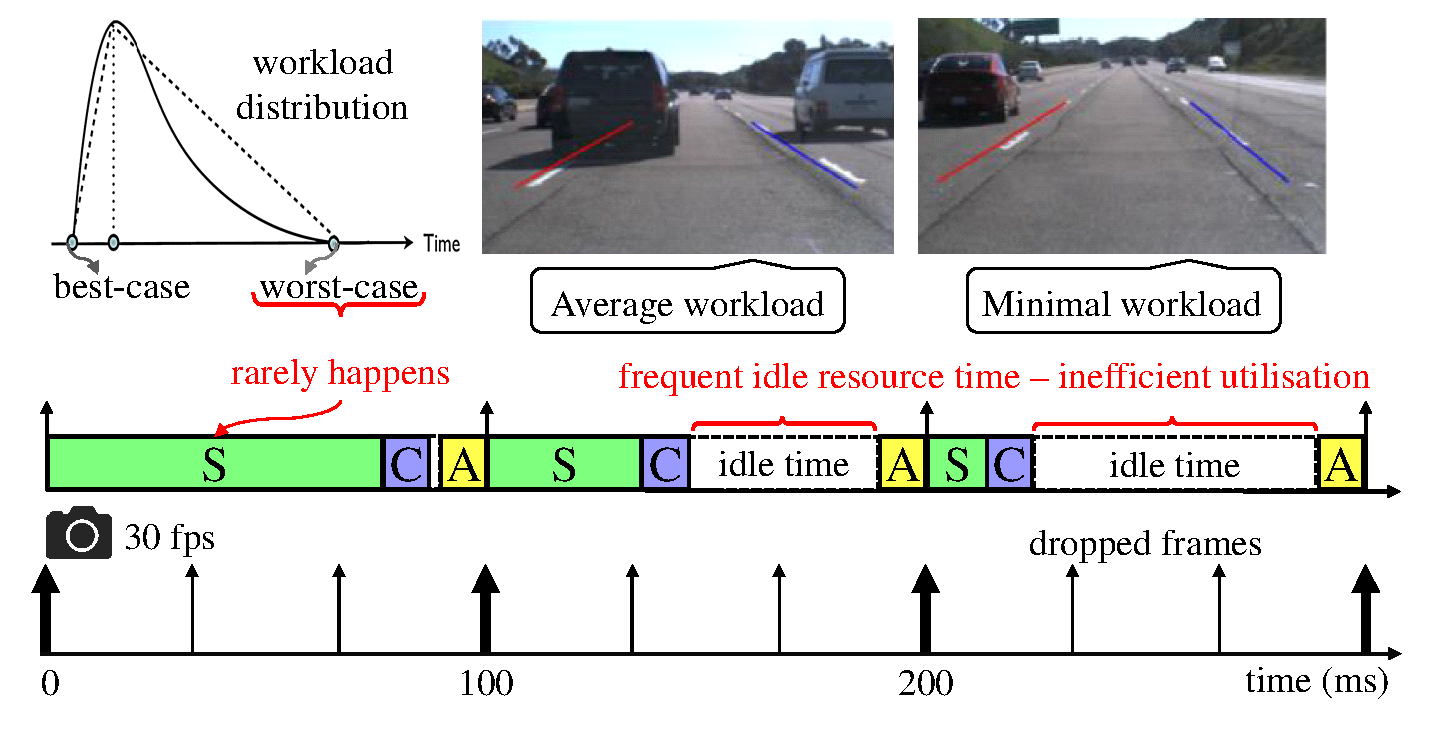
\includegraphics[width=\textwidth]{images/workload_IBC.eps}
    }
    \caption{Illustration of \gls{ibc} system implementation and challenges for \gls{lqr} control design considering worst-case workload. \taskS: sensing and image processing, \taskC: control computation and \taskA: actuation, see Fig.~\ref{fig:ch3_IBC_block_diagram}. (Adapted from Fig.~\ref{fig:ch5_intro}, for readability.)}
    \label{fig:ch3_workload_IBC}
    \vspace{-2em}
\end{figure}

The workload variations can, however, be statistically analysed, e.g., as a PERT distribution~\cite{adyanthaya2014robustness} or \gls{dtmc}~\cite{welton2005estimation}, from observed data and can be modelled as workload scenarios (explained in Chapter~\ref{chap:parallelisation}).
 The workload scenarios can be modelled (e.g. as a task graph or a dataflow graph), analysed (for timing) and then mapped to a multiprocessor platform. 
 A system scenario abstracts multiple workload scenarios having the same sampling period as determined by platform constraints.
 An optimal mapping and controller may then be designed for each system scenario. 
 
For efficiently designing \gls{ibc} systems, we should consider the workload variations and the given platform allocation. 
An ideal design approach should: (i) identify, model and characterise the workload scenarios; (ii) find optimal mappings for these workload scenarios for the given platform allocation; (iii) identify optimal system scenarios; and (iv) design a controller with high overall \gls{qoc} for the chosen system scenarios.
One of the critical aspects here is: what is a good metric to define the \gls{qoc} for the application? 
A vision-guided braking application requires a fast settling time, whereas an automotive vision-based lateral control~\cite{taylor1999comparative} application requires to minimise the reference tracking error.

 Section \ref{chap:spadeoverview} introduces the \gls{spade} approach for designing \gls{ibc} systems.  \gls{spade} characterises a set of frequently occurring workload scenarios, identifies a set of system scenarios that abstract multiple workload scenarios based on platform constraints, and designs a switched linear control system for these system scenarios to improve \gls{qoc}.   
 However, if the number of switching subsystems is high, a challenge in \gls{spade} is the difficulty to guarantee stability for the resulting switched system~\cite{mohamed2018optimising, van2018data}.
In case of failure to guarantee stability, \gls{spade} as developed so far in the earlier chapters would result in \gls{lqr} control for the worst-case workload scenario.

The contributions of this chapter are as follows:
 \begin{itemize}
     \item We present an alternate controller synthesis method based on a \gls{mjls} formulation for the control design step in the full \gls{spade} approach of Chapter~\ref{chap:pipelined_parallelism}. Our synthesis method involves the following steps. (i) Modelling workload variations as a \gls{dtmc}, (ii) system scenario identification, and (iii) controller design and implementation. The motivation to choose the \gls{mjls} approach~\cite{costa2006discrete} over other standard sampled-data linear control design techniques~\cite{ogata1995discrete} is that it does not require us to know the exact sequence of incoming sample times due to the workload variations apriori.
     \item We provide design guidelines on the applicability of control design methods for given requirements, implementation constraints and system knowledge. For this, we compare the three control paradigms -- optimal control design using \gls{lqr}, switched linear control design~\cite{van2018data}, and controller synthesis using the \gls{mjls} formulation
     -- for \gls{ibc} system design with respect to \gls{qoc} while taking into account available system knowledge and implementation constraints, i.e., camera fps, platform allocation and mapping. 
     Note that we cannot compare with adaptive~\cite{goodwin1980discrete} or model predictive control~\cite{bemporad2002model} approaches since we do not know the exact sequence of occurrence of incoming sample times due to the workload variations apriori.
 \end{itemize}